\section{Exercise 4 and 5: Telegram Bot}

Following the guide, I developed a Telegram bot that uses the \textit{Open-Meteo API} to fetch the current weather in Padua. 

In particular, every time a user sends the command "\texttt{/getdata}", the Telegram bot makes an HTTP call to the \textit{Open-Meteo API}. Once it receives the response, it sends the data back to the user and stores the measurement in a local database.

All available commands are the following:
\begin{itemize}
    \item "\texttt{/start}": starts the conversation and shows the list of available commands;
    \item "\texttt{/getdata}": retrieves the current temperature in Padua;
    \item "\texttt{/history}": returns the last 10 measurements;
    \item "\texttt{/average}": returns the average temperature over all measurements stored in the database;
    \item "\texttt{/max}": returns the maximum temperature stored in the database;
    \item "\texttt{/min}": returns the minimum temperature stored in the database.
\end{itemize}

The code of the bot is available at the following link: \url{https://github.com/lalb03/Assignments-AIoT-2025-26/blob/b01b02599151ea6dd1423e50dac6728c923c3610/Telegram_bot/tel_ex-2.py}
\bigskip

In the following page, you can find a screenshot of a conversation with the bot.
\begin{figure}[h!]
    \centering
    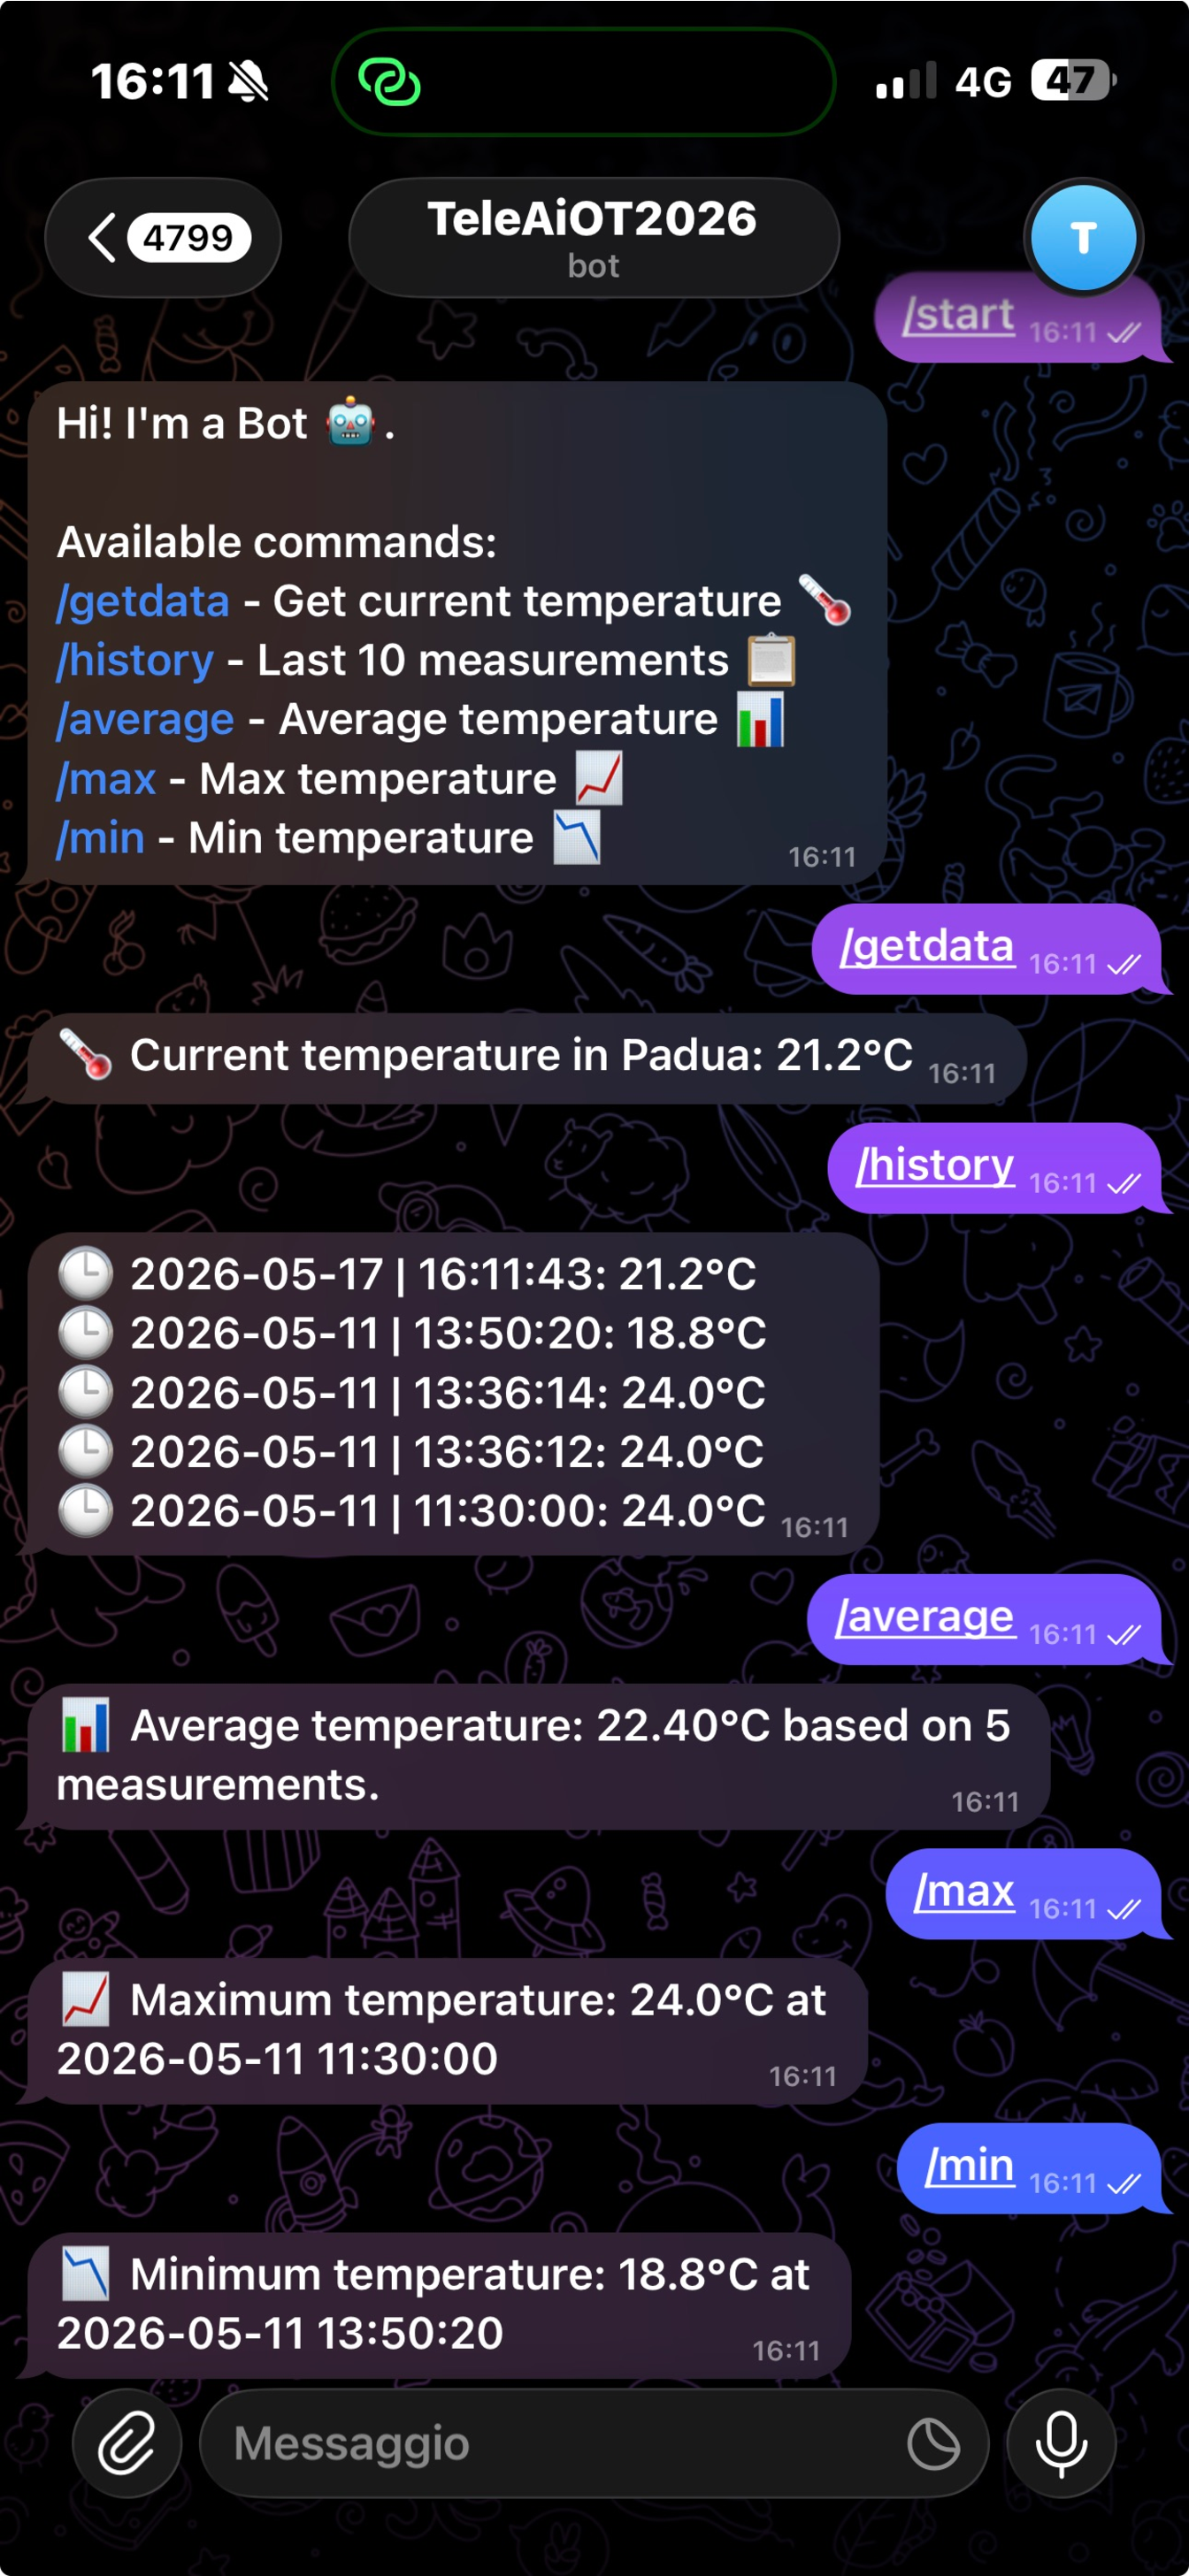
\includegraphics[width=0.5\linewidth]{Resources/Screenshot_chat.pdf}
    \caption{Screenshot of a conversation}
\end{figure}


